\documentclass[10pt]{report}
\usepackage{lingmacros}
\usepackage[normalem]{ulem}
%  Title Formatting 
\usepackage{titlesec}
% Removes paragraph indenting
\usepackage{parskip} 

% Figure labeling
\usepackage{hyperref}

\usepackage{amsmath}

% Font
\usepackage{tgpagella}

% Inline code
\usepackage{listings, lstautogobble}

\usepackage[labelfont=bf, labelsep=period]{caption}
\usepackage{graphicx}
\graphicspath{ {./images/} }

% Makes citations superscript
\usepackage[superscript,biblabel]{cite}
\usepackage{url}
\urlstyle{same}

\titleformat{\chapter}[block]
{\normalfont\huge\bfseries}{\thechapter.}{1em}{\Huge}
\titlespacing*{\chapter}{0pt}{-19pt}{0pt}

\lstset{language=Java,
	showstringspaces=false,
	breaklines=true,
	frameround=ffff,
	frame=single,
	autogobble=true
}


\begin{document}
	\begin{titlepage}
		\begin{center}
			\Large
			\textbf{Procedural Content Generation Using Noise}
			
			\vspace{1.5cm}
			\normalsize
			\textbf{Michael Li}
			
			\vfill
			
			\textbf{DRAFT 3.1.3}
			
			\uline{Dianne Hansford, Ph.D \hfill Director}
			\vspace{1cm}
			
			\uline{Yoshihiro Kobayashi, Ph.D \hfill Second Committee Member}
			
			\vspace{3cm}
			
			
\includegraphics[scale=.5]{asu_barretthonors_horiz_rgb_maroongold_600ppi}
			
			\vspace{1.5cm}
			Ira A. Fulton Schools of Engineering
			
			School of Computing, Informatics, and Decision Systems Engineering
			
			Spring 2021
			
		\end{center}
	\end{titlepage}
	
	\chapter*{Abstract}
	
	\addcontentsline{toc}{chapter}{Abstract}
	Procedural content generation is a method of creating data algorithmically using controlled randomness. These algorithms can be used to generate complex environments as opposed to manually creating environments, using photogrammetric techniques, or other methods. Procedural generation can use a variety of techniques including fractals, noise, cellular automata, and deep learning. This paper will survey various procedural algorithms, how they work, and briefly cover some examples and the history.
	
	\clearpage
	
	\tableofcontents
	
	\clearpage
	
	\let\clearpage\relax
	\chapter{Introduction}
		
		Procedural generation is an often hidden, yet common feature among digital content, as it automates the creation of large amounts of data. Often, this is hidden in the backgrounds of movies and video games, as well as other art -- adding subtle texture and variation. Procedural generation has many possible outputs, with some examples being the generation of stories, histories, particle effects, and characters. One of the most famous cases of procedural generation for entire worlds is Minecraft \cite{minecraft-gen}. Other examples of procedural generation's varied uses include games such as The Elder Scrolls II: Daggerfall, which employs various forms of procedural generation to determine the location of non-player characters, the layout of dungeons, as well as the terrain itself \cite{daggerfall}. In more complex cases, procedural generation is used to create fake histories, with the more well-known example of Dwarf Fortress \cite{df-dev}. However, procedural generation's applications are not only limited to games. In The Lord of the Rings, many of the scenes with large amounts of characters were created using procedural generation, ensuring individual animations of the slightly differentiated characters \cite{massive}.
		
		This paper surveys various procedural algorithms and examples of the procedural generation of content and their applications in generating geological formations and the surrounding terrain. Procedurally generated content (PGC) refers to the use of computers to algorithmically create data using a pseudo-random procedural algorithm, which is then interpreted into content. Some procedural algorithms to create content includes noise, fractals, as well as cellular automata. These algorithms can be mixed and matched in any number of ways to fine-tune different outcomes, or to add variety to content. To qualify as PGC, the algorithm to create data must be modifiable and controllable, while the results from the algorithm must be reproducible. The reproducible criteria for PGC can be fulfilled by the use of deterministic random number generators (See \autoref{sec:rng}), but some forms of procedural algorithms are majority governed by randomness. The modifiable criteria is fulfilled by the use of parameters to modify the algorithm. A deterministic system is a system in which no randomness is involved, while a stochastic system is one that can be described by a random probability distribution. While these concepts may seem to be mutually exclusive, they occupy different portions of the overall procedural generation pipeline, allowing them to co-exist. A geological formation, is a body of rock that possesses some degree of internal consistency or distinctive features \cite{2005}. This allows geological formations to be separate from the region it is placed in while still being a landmark for the region as a whole. Just as sand is individually different at a small scale, so too is the data created by procedural generation. However, when viewed as a whole, there is little difference between each grain. This necessitates user control and adjustments in order to make a region stand out versus another, with the use of landmarks or geological formations.
		
		\section{Motivation for Procedurally Generated Content}
		
		\section{Fundamentals} \label{sec:rng}
		
		PGC is often dependent on the use of random numbers. Random numbers may be generated through non-deterministically through the use of unpredictable physical processes, and deterministically using an algorithm \cite{rng}. These methods are also known as random bit generators, Non-deterministic Random Bit Generator (NRBG) and Deterministic Random Bit Generator (DRBG), respectively. One example of an unpredictable physical process to generate non-deterministic random numbers is through using radio receivers to pick up atmospheric noise \cite{random-org}. A NRBG measures a random physical process and compensates for potential biases to generate a random number. For deterministically generated random numbers the random numbers are algorithmically determined using an input value (also known as a seed). A DRBG is an algorithm to generate a sequence of numbers whose distribution approximates a sequence of random numbers. The algorithm to create these numbers is static -- by inputting a seed, the same sequence of random numbers will always be created. This concept of repeatablity is shared between PGC and DRBG's. DRBG's are also known as pseudorandom number generators, and their generated numbers are described as pseudorandom because they only approximate randomness -- the deterministic portion of the algorithm makes true randomness in this context impossible. PGC algorithms follow the same methodology as DRBGs. PGC also often uses a seed for the procedural algorithm. In procedural generation, the seed ensures the criteria for procedural generation to be reproducible, acting as a soft limit to the amount of randomness that can be created, since seeds are often relatively short in size. This seed number as the starting point, will only have meaning in the context of the same algorithm it is being used in -- changing the algorithms and/or manipulating the seed will change the entire output. This ensures regularity and controlled randomness to the PGC in a static environment, since any input number will result in the same set of outputs using the same procedural generation methodology. By taking an input seed, it will be modified using an procedural algorithm to obtain the output, possibly using additional random numbers created after the original seed. By using a DRBG, the creation of these numbers will be static, as the "seed" for a DRBG will determine the sequence of random numbers that it returns.
	
		\section{Methods Overview}
		This section will briefly cover some procedural algorithms as well as an introduction to their methods and usage. These will be further elaborated on later, with additional details in their application and quirks in PGC. 
		
		Noise is a method of creating PGC, using the seeding method to manipulate and control the outcome. Lattice gradient noise is a commonly used and widespread form of noise. This form of noise creation works off of the premise of an integer lattice -- a regularly spaced array of points in a square array \cite{integer-lattice}. One of the most well-known applications of this is Perlin noise, notably developed for use in Tron \cite{tron} to create textures to allow for more realistic, interesting and believable effects and images \cite{ken-perlin}. Pseudo-random numbers (referring to numbers created by a DRGB) are generated and evenly distributed across this lattice, then a low-pass filter is applied to smooth the edges between each of these points. A low-pass filter in this application helps to smooth the created lattice by averaging nearby values, shown in \autoref{fig:lpf}. 
		
		\begin{minipage}{\textwidth}
			\centering
			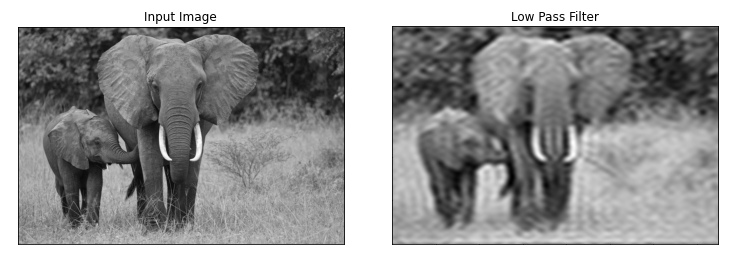
\includegraphics[scale=0.5]{lowpass}
			\captionof{figure}{Low-pass Filter Effect}
			\label{fig:lpf}
		\end{minipage}
		
		This creates a blurring effect, with fewer large value changes. This gradation between each of the lattice points reduces the randomness present in the lattice. The result is an image such as the one shown in \autoref{fig:noise-ex}.
		
		\begin{minipage}{\textwidth}
			\centering
			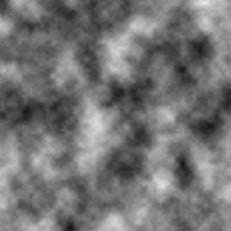
\includegraphics[scale=1]{lect14-perlin}
			\captionof{figure}{Perlin noise example. \cite{noise-ex}}
			\label{fig:noise-ex}
		\end{minipage}

		Fractal-based algorithms are another approach at creating PGC. Fractals are mainly characterized by their self-similarity. This means that the parts of the whole fractal contain the same characteristics. Fractals and the subsequent geometric shapes that can be created from fractals can be used to describe nature. Fractal geometry applied to landscapes began with studies of map data and research on the similarities between fractals and the data. Fractals prove as a relevant approach to representing geographical data due to the self-similarity and the subdivision of space, made easier by fractal surfaces \cite{doi:10.1111/j.1467-8306.1987.tb00158.x}. This provides a method of predicting the appearance and geometry of landscapes being studied. The technique works primarily from the subdivision of space combined with random numbers for each of the vertices created from the subdivision of space \cite{fractal-land}. In \autoref{fig:spatsub}, the four corner points act as the initially chosen vertices, and the vertices in the newly created plus shape are the vertices to randomly raise or lower. 
		
		\begin{minipage}{\textwidth}
			\centering
			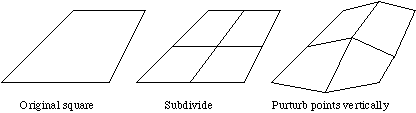
\includegraphics[scale=1]{landscapes}
			\captionof{figure}{Spatial Subdivision.\cite{fractal-land} Original figure show on the left. In the middle, the figure is subdivided, then on the right the points resulting from the subdivision are perturbed vertically.}
			\label{fig:spatsub}
		\end{minipage}
		
		Similarly to Perlin noise, this technique often utilizes a seed random number to start from, to make the results reproducible. However, while fractals are very computationally efficient, the parameter that makes this seed is very sensitive to change. Very small changes will completely change the features of a map designed this way.
		
		\begin{minipage}{\textwidth}
			\centering
			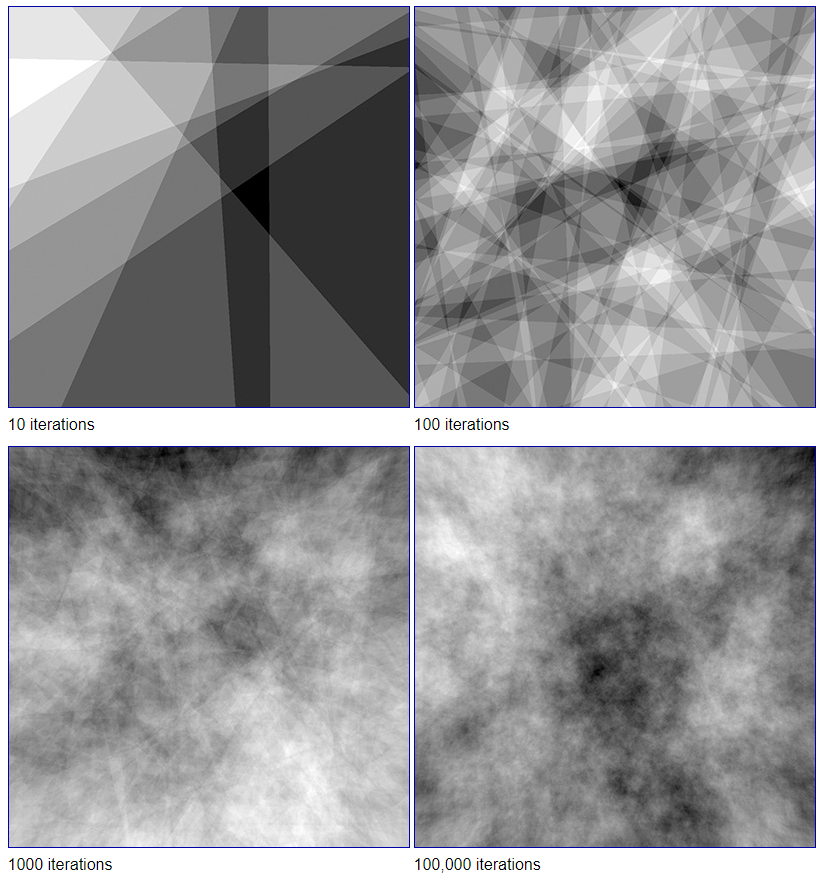
\includegraphics[scale=.4]{fractal-noise}
			\captionof{figure}{Fractal procedural generation example \cite{fractal-land}}
			\label{fig:fractal-land}
		\end{minipage}
		
		Another method of generating terrain and other features such as caves \cite{10.1145/1814256.1814266} revolves around the use of cellular automata. A cellular automata is a model of a system of cell objects with three characteristics. The cells must be placed on a regularly spaced grid, regardless of dimensionality. In addition, these cells must each have a state, which can describe any number of features for each individual cell. Lastly, each cell must have a neighborhood. While typically a neighborhood is composed of only the adjacent cells, it can be defined in any number of ways. This approach relies on having the information of neighbors and the states of their neighbors to determine surrounding cells to then modify their states \cite{nature-of-code}. This can be used in conjunction with a tiling system to procedurally generate geological features and the surrounding terrain.
		
		\begin{minipage}{\textwidth}
			\centering
			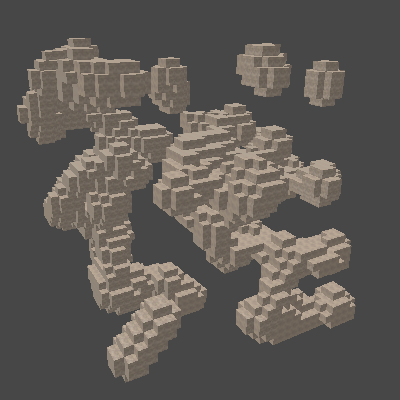
\includegraphics[scale=.75]{cellular-automata-cave}
			\captionof{figure}{An example of three-dimensional cellular automata cave generation \cite{bergauer_prozedurale_nodate}}
			\label{fig:ca-cave}
		\end{minipage}
		
		\section{Representing Data}
	
		Representing the data generated procedurally is another task with a variety of solutions. Some of these methods include pixel-based methods, polygons, and voxels. One common, simplistic way to represent the data generated is to use ASCII characters, or other types of two-dimensional data such as colored pixels to convey the scene that is being represented. In the case of Dwarf Fortress, the use of ASCII symbols is used to represent the elements within the game, shown in \autoref{fig:asciidf}.
		
		\begin{minipage}{\textwidth}
			\centering
			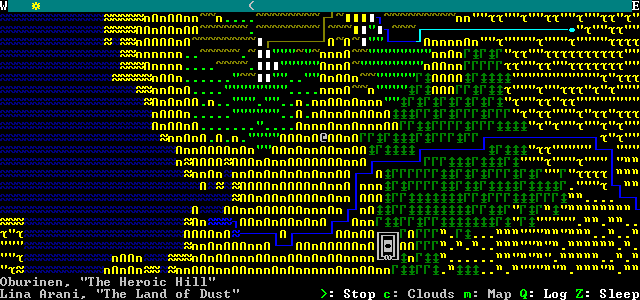
\includegraphics[scale=.5]{dwarf_fortress}
			\captionof{figure}{ASCII representation of PGC. \cite{df-dev}}
			\label{fig:asciidf}
		\end{minipage}
		
		Polygonal meshes are a way of representing three-dimensional objects. These are created through polygons (typically triangles) joined by at least two vertices. These polygons are then represented by the coordinates of the vertices that compose them, while the space between the vertices acts as the viewable portion.
		
		Voxels represent a volume element in space. These are placed in a regularly spaced grid of similar values. These values in space can contain multiple data points, such as opacity, color, geometry (for example, cubes), among other things. Voxels are represented by their position relative to other voxels, allowing for easier representation of layers of geometry. 
		
	\vspace{10pt}
	\let\clearpage\relax
	\chapter{History}
	
		\section{Fractals}
		Brownian motion was one of the starting points for procedural algorithms, used to describe the random motion of particles within water. Robert Brown first described this natural phenomenon in 1827. The stochastic process behind Brownian motion was later mapped into an algorithm almost a century later, a method called the Wiener process \cite{inbook}. A standard Wiener process on the interval \([0,T]\) is a random variable \(W(t)\), where \(t \in [0,T]\). This must satisfy the following:
		
		\begin{itemize}
			\item \(W(0) = 0\)
			\item \(For 0 \leq s < t \leq T\) 
		\end{itemize}
		
		\(W(t) - W(s) ~ \sqrt{t - s} N(0,1)\), where \(N(0,1)\) is a normal distribution with zero mean and unit variance. 
		
		\begin{itemize}
			\item For \( 0 \leq s < t < u < v \leq T\), \(W(t) - W(s)\) and \(W(v) - W(u)\) are independent.
		\end{itemize}
	
		On a computer, \(N(0,1)\) can be obtained by the use of a random method, as long as they meet the criteria \cite{wiener-process}. 
		
		\begin{minipage}{\textwidth}
			\centering
			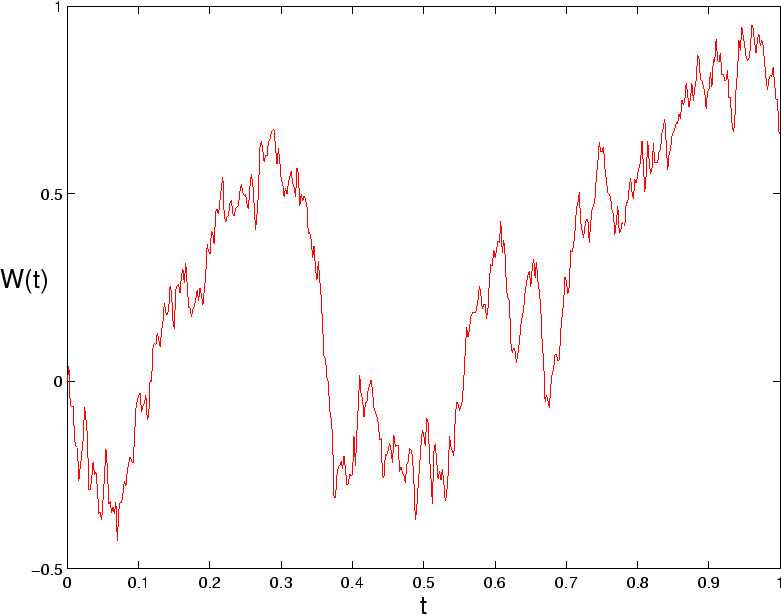
\includegraphics[scale=.3]{wiener-process}
			\captionof{figure}{A Wiener process \cite{wiener-process}}
			\label{fig:wiener-proc}
		\end{minipage} 
		
		The beginning of the use of fractals to describe landscapes did not coincide with the conception of the term "fractal" by Mandelbrot in the 1970s (See \autoref{sec:fractal}), but developed in the decades to come. This development in capturing surface topography was fueled by Mandelbrot's claim that all forms of nature can only be adequately described using fractals. While the potential of fractals to encapsulate and generate this geometry was noticed in the early 1990s, research at the time was still immature and unable to fully link the processes which create the forms captured by fractals. In terms of general landscapes, fractals were discovered to be able to imitate the self-similarity present in limited regions and limited ranges of scale in real landscapes. Some of the problems in furthering this research included the difficulty in researching and representing the dimensionality of natural terrain \cite{XU1993245}. Generating fractal structures ran into issues with processing time, causing a need for an alternative \cite{inbook}. However, this early PGC found its use in \emph{Star Trek II: The Wrath of Khan} \cite{startrek} to procedurally create imaginary planets. This technology was used later on in an accompaniment to a SIGGRAPH paper to demonstrate more of the ability of fractals. This set the stage for further use in movies such as \emph{The Last Starfighter} and \emph{Return of the Jedi} \cite{ibm-fractal}. 
		
		\section{Cellular Automata}
		
		During the development of fractals, cellular automata also were studied and gained traction. Cellular automata were originally proposed by John von Neumann, focusing on their structure in one and two dimensional grids. This idea was eventually extended into games by John Conway, with the motivation to design a simple set of rules to study the behavior of a population. By tuning different configurations, the "Game of Life" demonstrated a variety of growth patterns stemming from the initial population. Another example of the application of early cellular automata research to games was the \(\sigma(\sigma\textsuperscript{+})\) game, proposed by Sutner. This utilized the capabilities of cellular automata in a 2-d finite grid in order to have two players play against each other \cite{10.1145/349194.349202}.
		
		\section{Noise}
		
		In a similar period, Perlin noise was developed for use in the movie industry as well. It later became a foundation for many other procedural generation algorithms. It was developed in 1983 for use in the sci-fi movie Tron, to map textures onto computer generated surfaces for visual effects. Perlin noise has been used for many visual elements, ranging from the texture creation it was created for to particle effects such as fire, smoke and clouds, as well as landscapes and geological features. It has a variety of uses due to its ability to create a naturalistic appearance \cite{10.1145/325165.325247}.
		
		\section{Applications}
		One of the earliest usages of PGC in video games was in Rogue, in 1980 \cite{rogue}. This initial attempt at generating a dungeon in a random manner addressed some of the differences between procedural generation and purely random generation, by introducing some level of control to the designer. Rogue addressed this by using a three by three grid to generate the layout of the level, with hallways randomly connecting the rooms. These rooms would have a variable size to increase the variety of levels producible by the algorithm. This technique in particular, was created to address the memory constraints of computers at the time, as even with this more mathematical and less memory intensive approach, levels would need to be cleared from memory when moving on to the next one \cite{rogue}.
		
		% can add more here if have time...

	\vspace{10pt}
	\let\clearpage\relax
	\chapter{Procedural Generation Methods}
		\section{Cellular Automata}
			Cellular automata are composed of n-dimensional grid of uniform cells, each containing a state. For example, a one-dimensional cellular automata would be a row of cells. These cells are governed by a certain set of rules which are dependent on the neighborhood of cells, which can have a multitude of definitions. Typically, a neighborhood is just defined as the adjacent cells. The rules of a cellular automata determine the state of cells in the next generation, which indicates the next step of the algorithm. Each generational step updates the state of cells according to the defined rules. In \autoref{fig:cell-30}, an example of cellular automata is shown, with each row representing an iteration of the algorithm.
			
			\begin{minipage}{\textwidth}
				\centering
				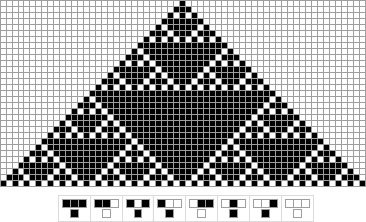
\includegraphics[scale=0.8]{rule-30}
				\captionof{figure}{1-Dimensional cellular automata example. Each row is an iteration, following the eight rules at the bottom \cite{cell-30}.}
				\label{fig:cell-30}
			\end{minipage}
		
			This algorithm follows the eight rules below the pyramidal structure, with the initial state consisting of an even padding of white cells surrounding one black cell. For cellular automata, the recursive nature of the algorithm causes the growth and evolution over time, as seen above. While this cellular automata example works based off of a neighborhood definition of just the adjacent cells, this definition is malleable, and controllable by the user, allowing for a wide variety of different outcomes with minor adjustments. Cellular automata's methodology is similar to other types of procedural algorithms, as the input state of the n-dimensional grid acts as the "seed" for the cellular automata. This can vary widely in output based on the set of rules and definition of neighborhood given. It can be seen in \autoref{fig:cell-30} that cellular automata are even capable of replicating the appearance of fractal structures, and mimic their recursive nature. Cellular automata can run into the issue of setting the initial input, as for physical computers, having an infinite input size is not possible. For this problem, there are three possible solutions. 
			
			\begin{enumerate}
				\item \textbf{Edges remain constant.} Edges will not be evaluated by the algorithm.
				\item \textbf{Edges wrap around.}
				\item \textbf{Edges have different neighborhoods and rules.} \cite{nature-of-code}
			\end{enumerate}
			
			While cellular automata can have a large variety of possibilities, the majority of simplistic rulesets will not produce satisfying outcomes. The different range of outcomes of cellular automata have been divided into four classes by Wolfram.
			
			\begin{enumerate}
				\item \textbf{Uniformity.} After a number of generations, every cell becomes constant.
				\item \textbf{Repetition.} Similarly to class 1, the cellular automata becomes constant, but the cell states themselves shift in a periodic pattern.
				\item \textbf{Randomness.} The cellular automata and the cells have no discernible pattern. 
				\item \textbf{Complexity.} The cellular automata will have repeating patterns, but the patterns location and place in the process itself will not have a pattern \cite{nature-of-code}. 
			\end{enumerate}

		\section{Fractals} \label{sec:fractal}
			Using fractal methods for PGC is another way of generating data. Fractals are objects with a recursive, or repeating, definition. These objects have a self similarity at different levels of magnification. For example, the Koch snowflake demonstrated one of the rules of fractals in a geometrical point of view. By repeating two rules, it was possible to generate complex shapes.
			
			\begin{enumerate}
				\item Draw an Equilateral triangle
				\item Replace all lines as follows, and repeat 2
			\end{enumerate}
		
			\begin{minipage}{\textwidth}
				\centering
				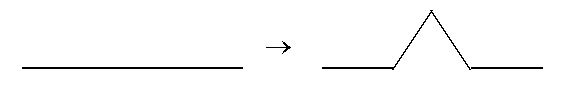
\includegraphics[scale=0.5]{m_reprule}
				\captionof{figure}{Rule of the Koch snowflake \cite{fractal-landscapes}.}
				\label{fig:m_reprule}
			\end{minipage}
		
			After several iterations of this rule, \autoref{fig:m_koch} is the result.
			
			\begin{minipage}{\textwidth}
				\centering
				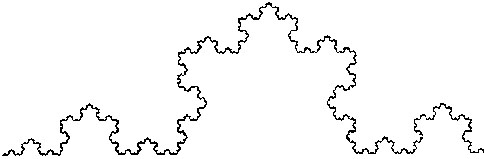
\includegraphics[scale=0.5]{m_koch}
				\captionof{figure}{Koch snowflake \cite{fractal-landscapes}.}
				\label{fig:m_koch}
			\end{minipage}
			
			To use fractals to generate geological formations, the initial fractal algorithm must be modified. While fractals can be used in their base form for PGC, additional modifications to add controlled randomness are necessary to incorporate features from more realistic landscapes. By using multiple rules of replacement, rather than the single one from the Koch snowflake, through a deterministically random selection, a more naturalistic output can be achieved. One example of generating these fractal surfaces is through displacement noise. One example of the effect of displacement noise can be seen in \autoref{fractal_displacement1}, where a fractal displacement noise pattern is added to an image to distort the image. 
			
			\begin{minipage}{\textwidth}
				\centering
				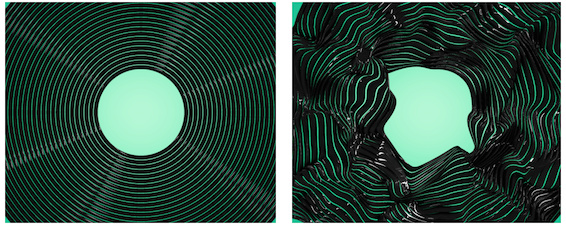
\includegraphics[scale=1.0]{fractal_displacement1}
				\captionof{figure}{Example of fractal displacement to distort an image. \cite{fractal_displacement1}.}
				\label{fig:fractal_displacement1}
			\end{minipage}
			
			An example recursive process for generating a fractal landscape involves the use of a heightmap (See \autoref{chap:storing_data}). For now, the initial starting point can be a grid of heights. Interpolation is a type of estimation for the value between two points, whether by averaging (linear interpolation), or some other function. The height of the points between these two values can be determined through interpolation, and a controlled random value can be added to them. 
			
			\begin{minipage}{\textwidth}
				\centering
				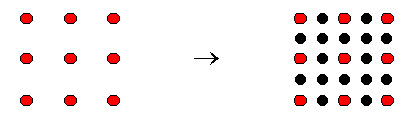
\includegraphics[scale=0.5]{m_alg1}
				\captionof{figure}{Interpolation of height values. Red points are the initial set, black points are the interpolated values to which the random values are added. \cite{fractal-landscapes}.}
				\label{fig:m_alg1}
			\end{minipage}
		
			One issue with this method of interpolating values is the creation of a relatively square region for each interpolation. This can me mitigated with the Diamond-Square fractal generation method, shown in \autoref{label}. By using multiple steps to find the values of the interpolated points, the square shape is minimized. 
		
			\begin{minipage}{\textwidth}
				\centering
				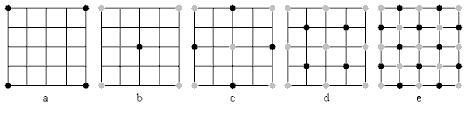
\includegraphics[scale=1.0]{diamond_square}
				\captionof{figure}{Steps are show left to right. The left-most figure shows the initial points to be interpolated. From there, gray dots represent the points from the previous step, while the black dots show the newly interpolated points. \cite{diamond_square}.}
				\label{fig:diamond_square}
			\end{minipage}
			
			Other methods of PGC are closely related to fractals as well. For example, while Perlin noise can be interpreted from a signals point of view, Perlin noise's output is also an example of the procedural generation of fractal surfaces using gradient noise \cite{fractal-landscapes}.
		
		\section{Noise}
			Noise refers a general concept of randomness often used in signals, but can also be applied as one of the procedural process used for PGC. In signals, noise is unpredictable and random, carrying no information. For PGC, noise can be modified to contain some level of consistency through the use of filtering and additional algorithms, to enable the noise to be interpreted in a useful manner. This difference can be seen in \autoref{fig:perlinnoise}, where the creation of noise is modified to produce a more interpretable and internally consistent output. 
			
			\begin{minipage}{\textwidth}
				\centering
				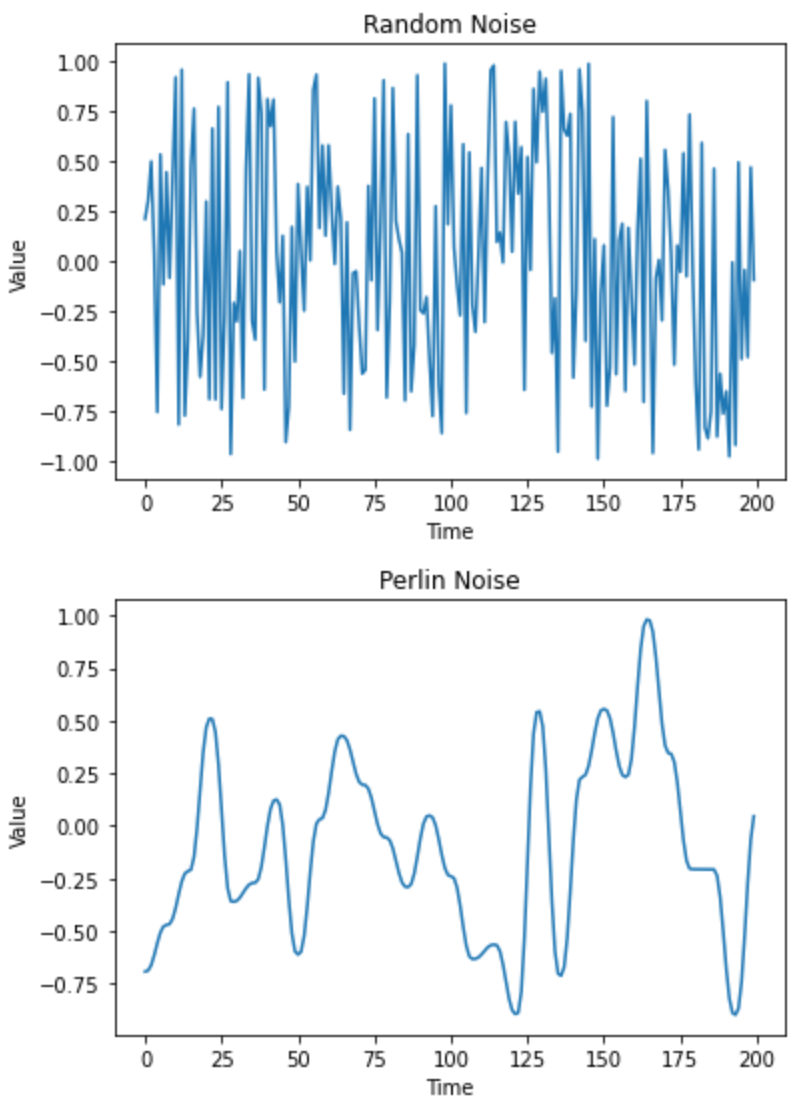
\includegraphics[scale=0.3]{perlinnoise}
				\captionof{figure}{Using the same set of input random numbers and the same algorithm, Perlin noise will always replicate this result.}
				\label{fig:perlinnoise}
			\end{minipage}
		
			Noise created in this manner runs into an issue of uniformity. In signal terms, this means that noise is band-limited, where almost all of the energy of the noise is concentrated in a very small part of the frequency spectrum. An example of is shown in \autoref{fig:bandlimit}, where applying a band-limiting effect smooths out the function.
			
			\begin{minipage}{\textwidth}
				\centering
				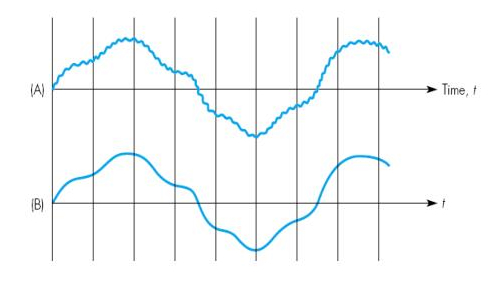
\includegraphics[scale=.5]{bandlimiting-filter}
				\captionof{figure}{Applying a band-limiting filter \cite{bandlimiter}}
				\label{fig:bandlimit}
			\end{minipage}
			
			The high and low frequencies of the original image would be blended out, and only the band-limited output image would remain, where the high and low frequencies contribute less to the total energy \cite{making-noise}. This can be mitigated by the use of layering differing octaves of noise to increase the amount of variation given by the noise. The term octave is borrowed from music, but when used in this context refers to the use of multiple noise functions combined, in order to create a more varied result with identifiable features. In \autoref{fig:perlin_octaves}, this effect of combining multiple octaves of noise can be seen.
			
			\begin{minipage}{\textwidth}
				\centering
				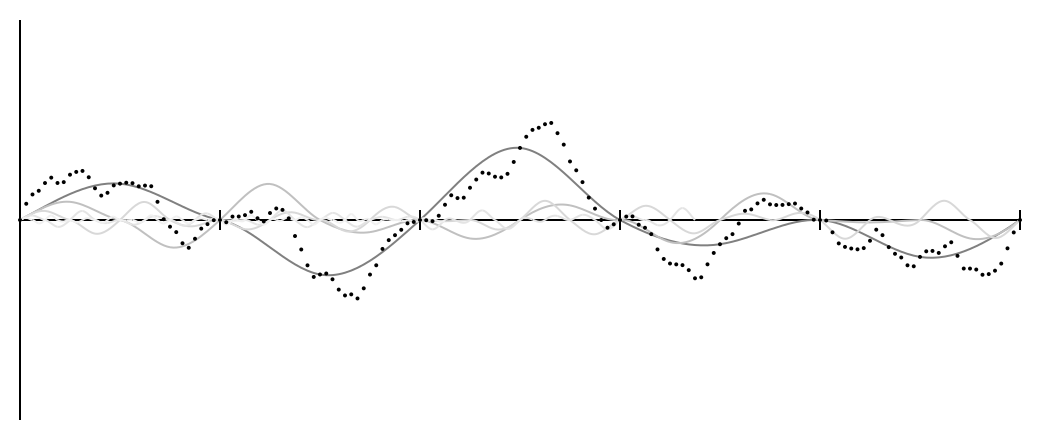
\includegraphics[scale=.4]{perlin_octaves}
				\captionof{figure}{Multiple Perlin Noise octaves combined. The dotted graph is the resultant noise.\cite{perlin-octaves}}
				\label{fig:perlin_octaves}
			\end{minipage}
	
			\subsection{Perlin Noise}
		
				One example of generating noise is through the use of the Perlin noise algorithm, named after Ken Perlin. The original implementation of Perlin noise was to create representations of various textures for objects, as well as representations of clouds, fire, water and stars among other things \cite{10.1145/325165.325247}. In other words, given an input point P, look at the surrounding points on the grid. In one dimension, this would be a series of line segments. 
				
				\begin{minipage}{\textwidth}
					\centering
					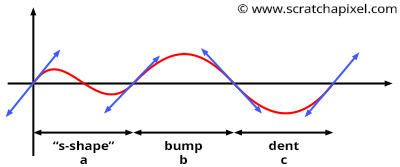
\includegraphics[scale=.5]{noise-value-vs-perlin3}
					\captionof{figure}{Perlin Noise gradients in one dimension \cite{pn-2}}
					\label{fig:pnoise1d}
				\end{minipage} 
				
				In two-dimensions there will be four points, due to the surrounding unit square, in three-dimensions there will be eight, due to the surrounding unit cube. Similarly to how in two dimensions space is parameterized by a lattice of integer squares, in three-dimensional space it is parameterized by a series of cubes. As Perlin noise scales up, this n-dimensional square/cube grows larger and larger in complexity, increasing the run time. For each of these surrounding grid points, Q, a pseudo-random gradient vector, G is chosen. This gradient is pseudo-random because, while the initial determination of the gradient vector's value is randomized, when inputting the same grid point the same gradient vector is chosen. In the calculation of Perlin noise, all of the points on the grid are located at zero. This attribute of Perlin noise can be seen in \autoref{fig:pnoise1d}. From there, the inner product is calculated between all of the surrounding grid points, the chosen point, and the gradient vectors. This results in \(G * (P - Q)\), giving 2\textsuperscript{n} values, where n represents the dimensionality of the grid. Then, interpolate between the values down to P, using an S-shaped cross-fade curve to weigh the interpolation in each dimension. This equation is shown below.
				
				\begin{lstlisting}[language=C]
					3t^2 - 2t^3
				\end{lstlisting}
				% cite? https://mrl.cs.nyu.edu/~perlin/doc/oscar.html#noise
				
				This was the original equation used for Perlin noise, but has since been superceeded. One of the problems with the previous equation used was that the second derivative of the function, \textbf{6-12t} is not zero at either \textbf{t=0} or \textbf{t=1}, causing discontinuities in the noise. Some of the effects of this are shown in \autoref{fig:pnartifact}. This led to the equation shown below to be used. 
				
				\begin{lstlisting}[language=Java]
					6t^5 - 15t^4 + 10t^3
				\end{lstlisting}
				% cite? https://mrl.cs.nyu.edu/~perlin/noise/
				
				This new equation led to an approximate ten percent speed increase compared to the original implementation. 
				
				\begin{minipage}{\textwidth}
					\centering
					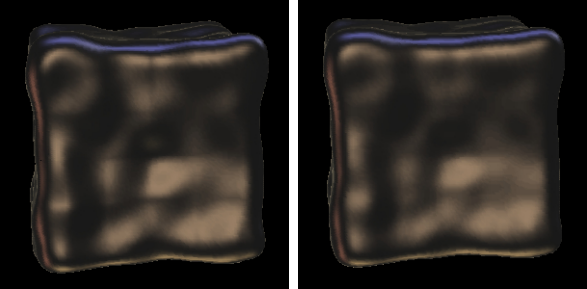
\includegraphics[scale=.5]{s-curve}
					\captionof{figure}{Removal of artifacting at t=0 and t=1 from revised interpolation function \cite{10.1145/566654.566636}}
					\label{fig:pnartifact}
				\end{minipage} 
				
				While Perlin noise saw great success, it was succeeded by algorithms such as Simplex noise, designed to alleviate some of the problems with Perlin noise. This included the computational complexity and the artifacting in the noise created. The artifacting in the noise appears from the necessity for the gradients to pass through zero, as shown in \autoref{fig:pnartifact}. This causes unavoidable artifacting in the noise. In addition, while Perlin noise's computational complexity is acceptable when in three-dimensional space and lower, it suffers greatly from increasing the dimensionality further.
		
	\vspace{10pt}
	\let\clearpage\relax
	\chapter{Storing Data} \label{chap:storing_data}
	
		PGC has the advantage of being able to be recreated through the use of the correct seed and algorithm in many cases. Another common method of storing topological data is through the use of height maps. 
		
		\begin{minipage}{\textwidth}
			\centering
			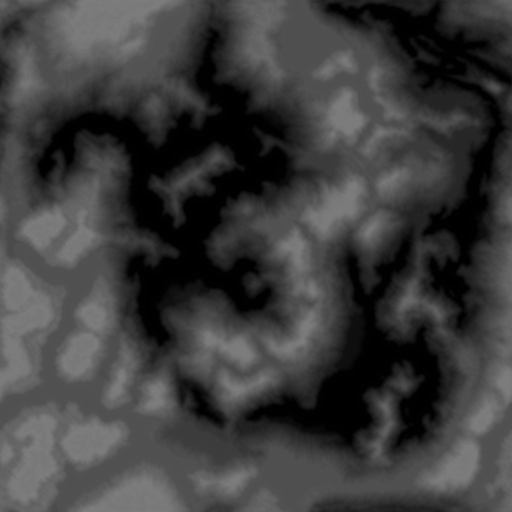
\includegraphics[scale=.5]{D10}
			\captionof{figure}{An example of a height map. \cite{voxel-space}}
			\label{fig:height-map}
		\end{minipage}
		
		The use of height maps is related to the development of some image based methods of rendering and displaying procedural content. A height map works by storing a single height value at each \[(x,y)\] coordinate. Height maps work similarly to topological maps, with an example of the latter shown in \autoref{fig:top-map}.
		
		\begin{minipage}{\textwidth}
			\centering
			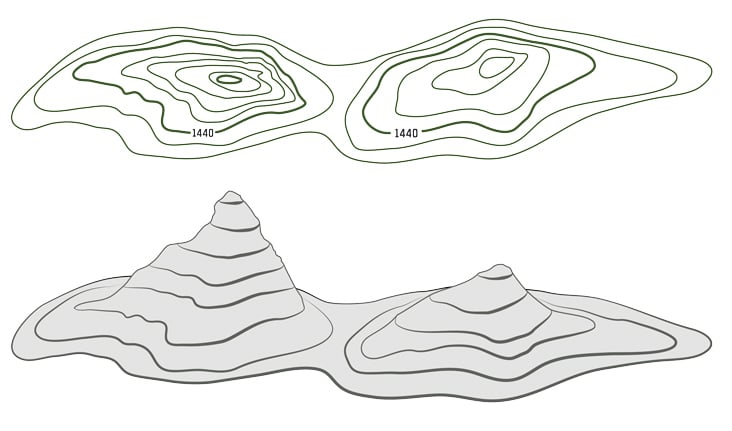
\includegraphics[scale=.5]{top-map}
			\captionof{figure}{A topological map is shown, with a corresponding three-dimensional representation of the map data below. \cite{top-map}}
			\label{fig:top-map}
		\end{minipage} 
	
		Height maps can be combined with a color map of the same dimensions, in order to map colors to each of the height locations. This effect can be seen in the voxel space rendering technique, shown in \ref{sec:imagebasedmethods} In terms of generating geological formations for landmarking a terrain, height maps add additional limitations on the possibilities. Height maps are unable to store multiple data values at each point, without significant complexity in interpreting the resultant data. This makes the generation of overhangs, arches, or any feature with protruding structures, difficult without additional data storage for these exceptions. A possible solution for this issue includes the storage of overhangs or similar features separately. Voxel based methods, or mesh based systems to store the terrain data instead have also been used.  
		
	\vspace{10pt}
	\let\clearpage\relax
	\chapter{Rendering and Display}
	
		\section{Image Based Methods} \label{sec:imagebasedmethods}
		
		Image based methods work by rendering based on the screen resolution of the output and the resolution of the input, rather than storing geometric positions. One example of image based rendering is the voxel space rendering system. The voxel space rendering system uses voxel raster graphics to display three-dimensional geometry with low memory and processing requirements. This was developed in the early 90's, involving a height and color map to position the pixels on the screen. While this technique was not historically used with noise generating algorithms, the rendering system fits the requirements for the use of techniques such as two-dimensional Perlin noise. By using Perlin noise, the height and color maps can be generated at run-time instead of being created beforehand. An example of this is shown in \autoref{fig:pnvs}. At the time, displaying complex height-maps in three-dimensions was difficult computationally, and the voxel space technique allowed this to happen.
		
		\begin{minipage}{\textwidth}
			\centering
			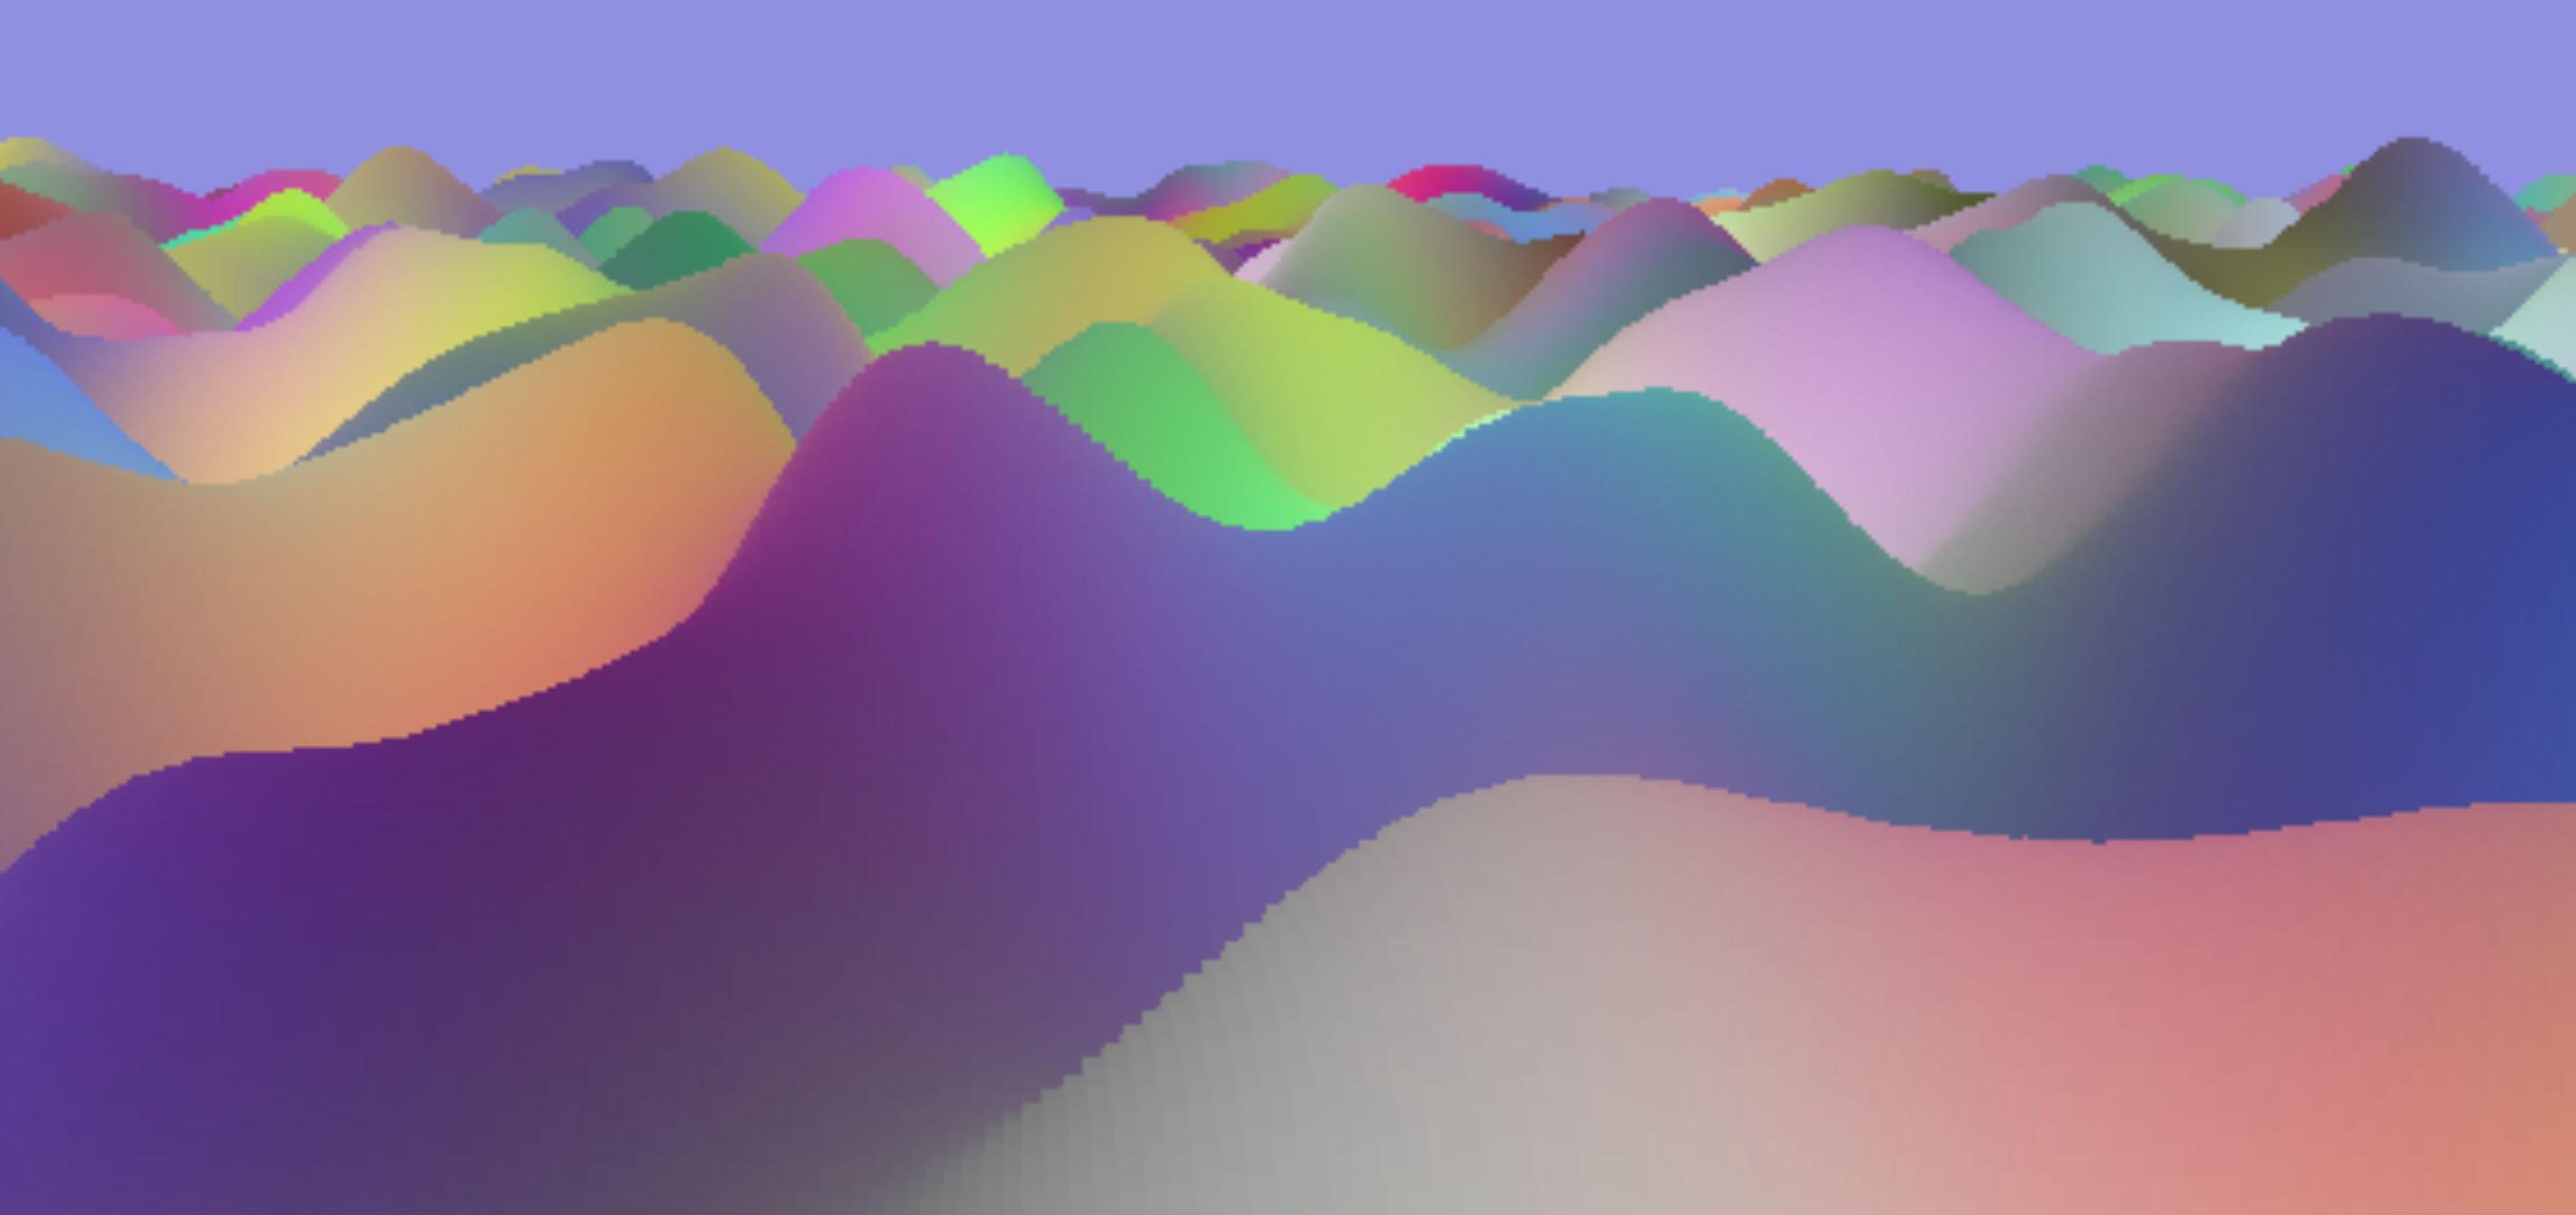
\includegraphics[scale=.15]{proc-voxel}
			\captionof{figure}{Rendering using the Voxel Space engine with a height and color map generated by Perlin noise.}
			\label{fig:pnvs}
		\end{minipage}
		
		The voxel space rendering engine originally utilized a pre-made height and color map to render from. This, combined with a tiling effect and knowledge of the field-of-view of the user's position allowed for a simplified three-dimensional rendering system. Starting from the furthest position to guarantee occlusion, a line on the map is determined in the triangular field of view. This is scaled with perspective projection, and a vertical line is drawn at every point on the screen from the section of the color map. The height of the vertical line is determined from the height drawn from the two-dimensional height map. Then, this is repeated until the entire field-of-view is drawn. This technique can be seen in \autoref{fig:vs-raster}. 
		
		\begin{minipage}{\textwidth}
			\centering
			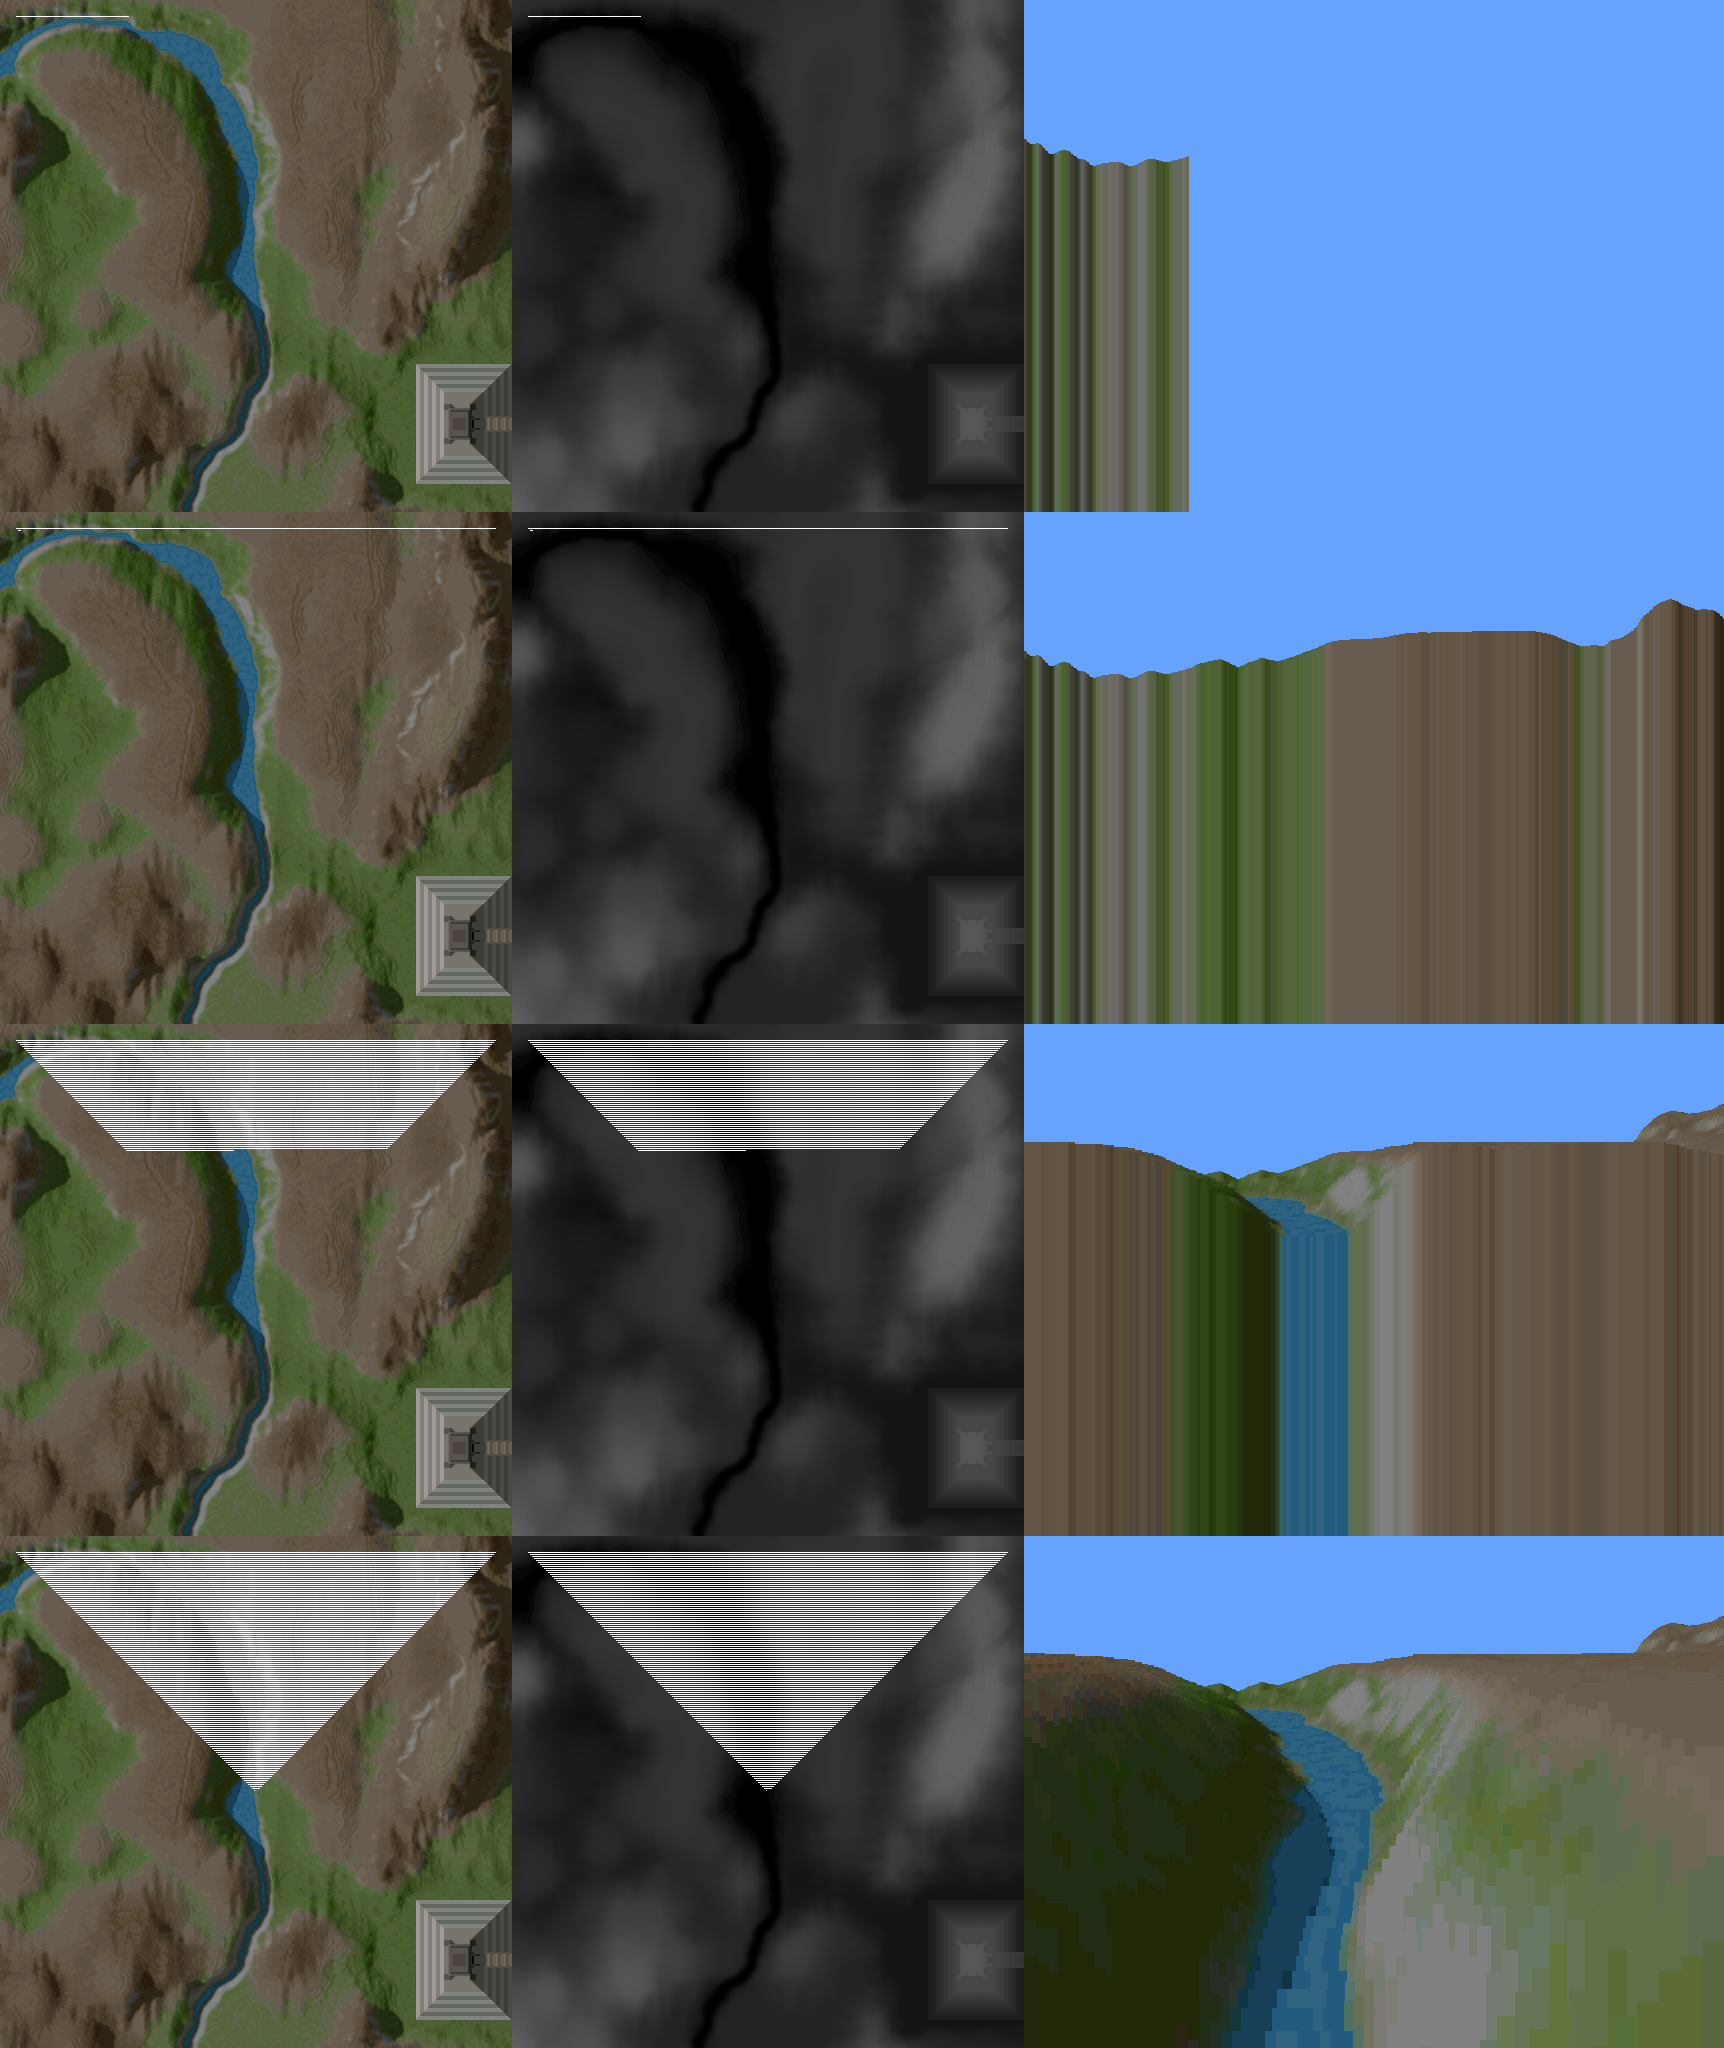
\includegraphics[scale=.2]{line-by-line}
			\captionof{figure}{Basic rasterization technique of the Voxel Space engine \cite{voxel-space}.}
			\label{fig:vs-raster}
		\end{minipage}
	
		This can be optimized with drawing from front-to-back with the addition of a y-buffer to determine the highest y position to draw. In this case, the y-buffer holds the highest y position, guaranteeing that the closest regions of the height map are displayed properly. However, the voxel-space rendering system has a downside of having fewer pixels to determine the colors and heights of closer landmasses. This creates a pixellated effect for the foreground, while the background is rendered in higher detail. This method can be seen in more detail in \autoref{fig:vs-patent}. 
		 
		\begin{minipage}{\textwidth}
		 	\centering
		 	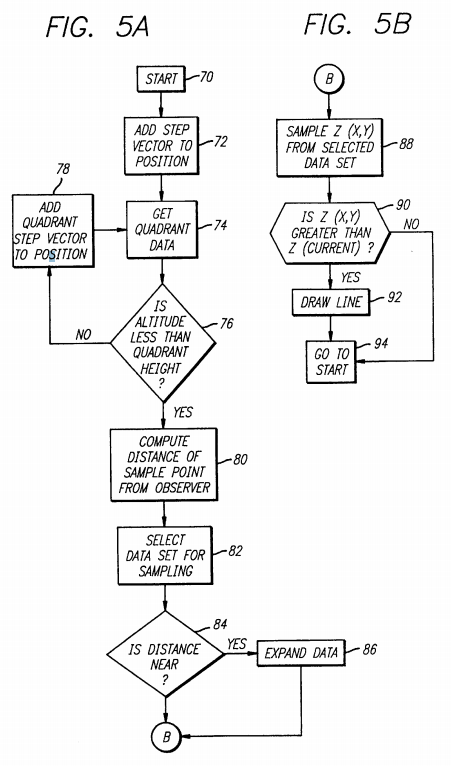
\includegraphics[scale=0.5]{US6020893A}
		 	\captionof{figure}{US Patent 6 020 893 \cite{US6020893}.}
		 	\label{fig:vs-patent}
		\end{minipage}
		
		This weakness can be mitigated in some effect by having multiple heightmaps of differing detail to draw from. This would mitigate some of the advantage of voxel space rendering in increasing the rendering time and processing required for the algorithm. In addition to the weakness in rendering closer objects, height maps are also unable to render more complex geological formations, such as caves, archways or overhangs. Later iterations of the voxel space rendering engine worked around some of these limitations by introducing rendering of both polygons and voxels. Another possible workaround to the low resolution of the voxel space rendering system would be using procedurally generated noise as the platform for creating height maps. By creating the height map dynamically from noise, the memory used for storing the program overall would be smaller, and the resolution would not be constrained, as for areas closer to the camera, the interpolation between the points of the noise map would just be decreased. 	
	
		\section{Polygononal Meshes}
	
		Using a polygonal mesh to represent an object is one of the most common methods of representing objects on a computer. A polygon is a planar shape, defined by connecting a series of vertices. A polygon mesh is composed of polygons, and is defined by three parts.
		
		\begin{center}
			\begin{tabular}{ l l } 
				V & a set of vertices (points in space)\\ 
				$E {\subset} (V x V)$ & a set of edges (line segments)\\ 
				$F {\subset} E^{\ast}$  & a set of faces \\
			\end{tabular}
		\end{center}
		% https://www.classes.cs.uchicago.edu/archive/2015/fall/23700-1/docs/mesh-notes.pdf
	
		These parts allow for the definition of a shape, composed of polygons. Triangles are the default polygon for use in polygonal meshes, the vertices composing the face of a triangle all have to occupy the same plane \cite{polygon}. By connecting the faces of multiple triangles, it is possible to assemble more complex shapes. For example, two right angle triangles connected along the hypotenuse edge will create a square, then six of these squares can be connected to form a cube. While this takes twelve triangles to represent, there are only eight unique vertices that need their position defined. An example of a polygonal mesh is shown in \autoref{fig:utah-teapot}.
		
		\begin{minipage}{\textwidth}
			\centering
			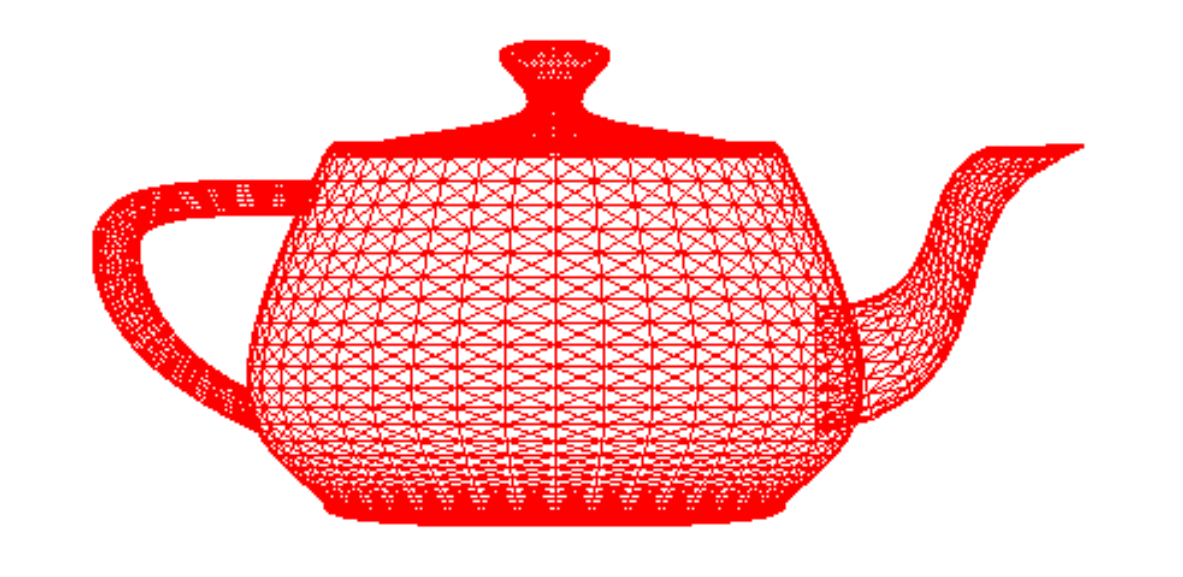
\includegraphics[scale=0.3]{utah-teapot}
			\captionof{figure}{A polygonal mesh of the Utah Teapot \cite{utah-teapot}.}
			\label{fig:utah-teapot}
		\end{minipage}	
		
		\section{Voxels}
	
		In contrast to polygons, voxels represent a volume element in space. Voxels act as a three-dimensional version of a pixel in space. While voxels are typically contained within a cubic cell in three-dimensions, they are not limited to this shape, and can have any number of shapes. These indivudual elements contain its position in space and another parameter or set of parameters, ranging from the color to the material to the texture data, among other possibilities. This allows for easier computation of the absence of terrain data, such as in caves or polygons. In terms of creating a cave, the points in space representing the cave just need to be removed, in contrast to the mapping required to store the vertices in space. 
		
		While the success of Minecraft has made it the atypical example of procedural generation rendered using voxels, the representation of voxels as cubes stacked in space is not accurate to the greater definition of the voxels being volume elements in space. Minecraft does use a voxel system to store the points in space as data, indexed by an YZX system for compression \cite{minecraft-voxel}. However, Minecraft's rendering system is based around a polygon system to display the individual blocks. 
		
		An example of a structure of representing voxel data is through the marching cubes algorithm. Each voxel (cube) in marching cubes is defined by the pixel values at the corners of the cube. These eight pixel values each contribute a single value, also known as a density value, with negative values indicating that the point is in empty space, and positive values indicating that the point is inside of solid terrain. A density value of 0, at the boundary of positive and negative, indicates the surface of the terrain. Along this surface is where the polygonal mesh is constructed \cite{marching-cubes}. At any voxel area contained within the eight points, the marching cubes algorithm allows generation of the correct polygons, outputting from zero to five polygons.
		
		To generate the polygons within the cell, the density values must be determined. The set of all corner vertices can be denoted as \(V = {v0,v1,v2,v3,v4,v5,v6,v7}\), where a positive density sets the vertex's bit to one, and a negative density sets the value to zero. 

		\begin{minipage}{\textwidth}
			\centering
			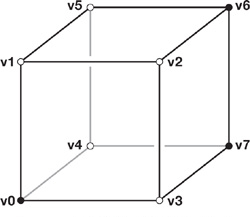
\includegraphics[scale=0.75]{01fig03}
			\captionof{figure}{A single voxel with example density values at the eight corner vertices \cite{marching-cubes}.}
			\label{fig:marching-cube}
		\end{minipage}
	
		\begin{center}
			\begin{tabular}{ l l } 
				\begin{tabular}{ l l }
					Case & = \\
				     	 & = \\
				     	 & = \\
				\end{tabular} 
				&
				\begin{tabular}{ r r r r r r r r }
					{ } v7$\vert$&v6$\vert$&v5$\vert$&v4$\vert$&v3$\vert$&v2$\vert$&v1$\vert$&v0\\
					{ } 1 $\vert$&1$\vert$&0$\vert$&0$\vert$&0$\vert$&0$\vert$&0$\vert$&1\\
					193&&&&&&&
				\end{tabular}
			\end{tabular}
		\end{center}
	
		These bit values can be concatenated with a bitwise OR operation to produce a single byte, in the range of 0-255. Two of these cases end up being trivial -- the concatenated value is 0 or 255, all the points are either inside of a solid terrain, or are in empty space. For the remaining configurations, there are only 14 unique combinations (shown in \autoref{fig:01fig04}) of the remaining 254 possibilities. This allows for the use of a look-up table to generate the polygons \cite{marching-cubes-paul}. 
		
		\begin{minipage}{\textwidth}
			\centering
			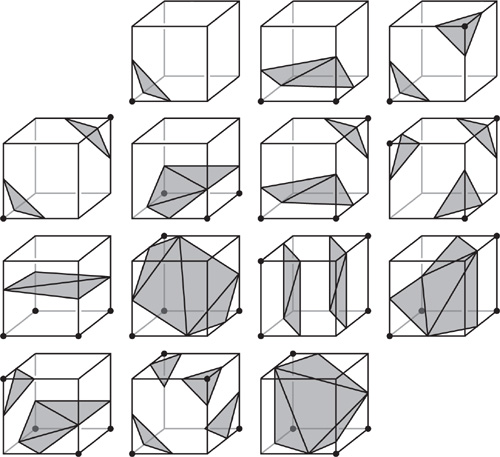
\includegraphics[scale=0.75]{01fig04}
			\captionof{figure}{A single voxel with example density values at the eight corner vertices \cite{marching-cubes}.}
			\label{fig:01fig04}
		\end{minipage}
	
		The placements of the vertices of each of these figures is determined by the density values for each of the corner points, by interpolating the value between these values.
		
	\vspace{10pt}
	\let\clearpage\relax
	\chapter{Development}

		\section{Areas of Research}
	
		An ongoing area of research for PGC is the introduction of neural networks as the framework, instead of more traditional algorithms or techniques. One example of this is the procedural generation of terrain via Tensorflow. This implementation was trained on a large data-set of terrain height maps, around 10,000, with the addition of satellite data to use for coloring. The specific neural network involved in the implementation was a Generative Adversarial network, which works on creating fake images, and attempting to discern between real and fake. By iterating this, the network will get better at both tasks, with the generator learning how to create more and more realistic images. For the problem of coloring the terrain, a style network was used to take two images and blend them to create an output image that looks like the content image, but with the style of the reference image. This technique is used in other applications, such as the neural networks trained on recreating photographs in a particular artist's style, shown in \autoref{fig:neural-style}. 
		
		\begin{minipage}{\textwidth}
			\centering
			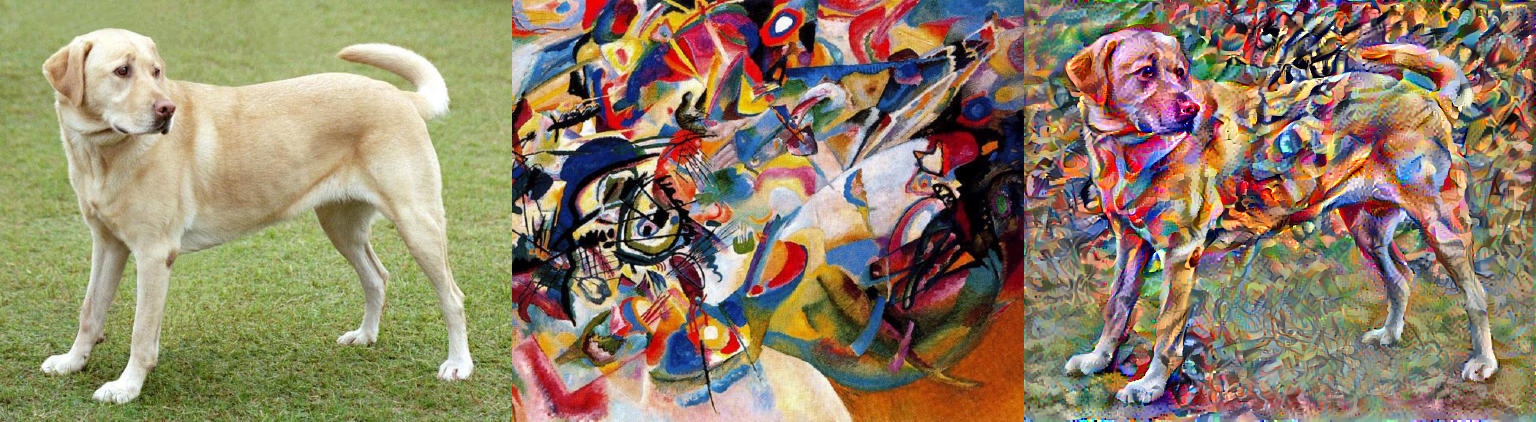
\includegraphics[scale=.3]{stylized-image}
			\captionof{figure}{An example of neural style transfer \cite{tf-style}}
			\label{fig:neural-style}
		\end{minipage}
	
		A kernel is part of image processing, and is applied to an image using convolutions. It is a \(n x n\) matrix, which is multiplied by over the pixels of an image, depending on the stride. \(n\) in this context provides the number of surrounding pixels, in a square formation for which to also draw values from for the new value of the pixel. The stride size refers to the distance the kernel moves for each convolution. If the stride size is too small, this can cause repeated multiplications across the image, a possible cause of artifacting. 
	
		\begin{minipage}{\textwidth}
			\centering
			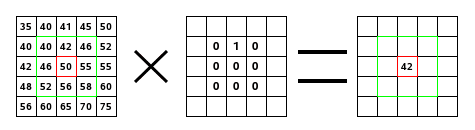
\includegraphics[scale=1]{convolution-calculate}
			\captionof{figure}{An of a kernel (pictured in the center as a 3x3 matrix) being multiplied at the target pixel in red. \cite{gimp}}
			\label{fig:gimp}
		\end{minipage}
		
		The initial processing pipeline for this image based deep learning algorithm utilized convolutional transpose to generate the output height and color-maps. However, this approach led to grid-like artifacting due to the misaligned output size compared to the kernel size. The solution used for combating this was bilinear sampling, by adding pixels from surrounding pixels to determine value rather than the kernels and strides. While the resultant height maps are impressive, additional research is likely required to determine differences between this approach and another approach such as Simplex noise. In \autoref{fig:dl-noise}, the results can be seen. 
		
		\begin{minipage}{\textwidth}
			\centering
			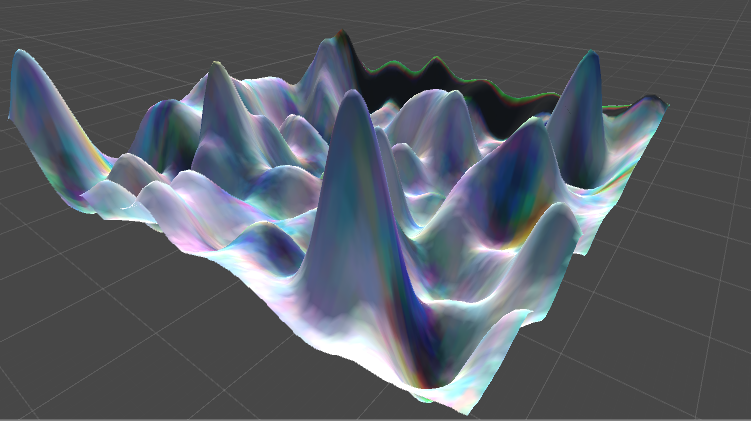
\includegraphics[scale=.3]{rolling}
			\captionof{figure}{Example of three-dimensional worlds created with deep learning \cite{nn-noise}}
			\label{fig:dl-noise}
		\end{minipage}
	
		The field of procedural content generation using machine learning is constantly evolving, as there are many different methodologies that have been applied to this task. The multitude of neural architectures allows for the tailoring of neural networks to different types of generated content, at the cost of necessitating large amounts of searching for the right architectures.
		
		\cite{Liu_2020}
		
		\section{Algorithm Advancements}
		
		Perlin noise was designed to address some of the limitations of the original Perlin noise. Since the original implementation of Perlin noise was constrained by the lattice gradient function creating directional artifacts, one of the goals of Simplex noise was to overcome this limitation. In addition, Simplex noise has lower computational complexity -- O(k\textsuperscript{2}) instead of O(2\textsuperscript{k})\cite{sheet-simplex}. Other benefits includes the capability to scale to higher dimensions, a well-defined and continuous gradient, as well as simpler implementation. Instead of the lattice gradients that Perlin noise works on, Simplex noise works based on simplex grids for which it was named after. This involves choosing the simplest, repeatable shape to fill a N-dimensional space. Another definition of a n-simplex would be it being the smallest figure that contains n+1 given points in n-dimensional space, while not lying in the space of a lower dimension. In one dimension, this works by choosing repeating line segments. In two dimensions, this becomes an equilateral triangle. In three dimensions, this becomes a trianglular pyramid, also known as a tetrahedron. From four dimensions and onward, this simplex becomes increasingly difficult to visualize. However, there is a pattern in the drawability of simplexes, by creating a new point and connecting it to all previously existing points.
		
		\begin{minipage}{\textwidth}
			\centering
			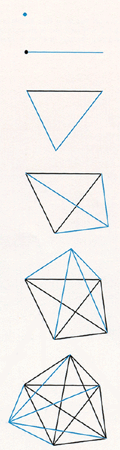
\includegraphics[scale=.75]{six simplexes}
			\captionof{figure}{The first six simplexes \cite{higher-dim-simplexes}}
			\label{fig:fig2}
		\end{minipage}
	
		The relative simplicity of the simplex shape in having as few corners as possible makes it a lot easier to interpolate values in the interior of the shape, relative to the hypercubes used in the original Perlin noise.
		In the original Perlin noise function, derivatives were used to compute the gradation between the points. This creates a large increase in computational complexity based on dimensionality. Simplex noise instead uses the summation of kernel values to determine the point's value. To generate the Simplex noise, the value for any point in space must be determined. In two dimensional space, this means skewing the coordinate space along the main diagonal, transforming the squashed equilateral triangles into right-angle isosceles triangles. From there, determining the location is made more simple, as just the integer part of the coordinates is needed for each dimension. Beyond two dimensions, the visualization becomes more difficult, but the methods remain the same.  
		
		\begin{minipage}{\textwidth}
			\centering
			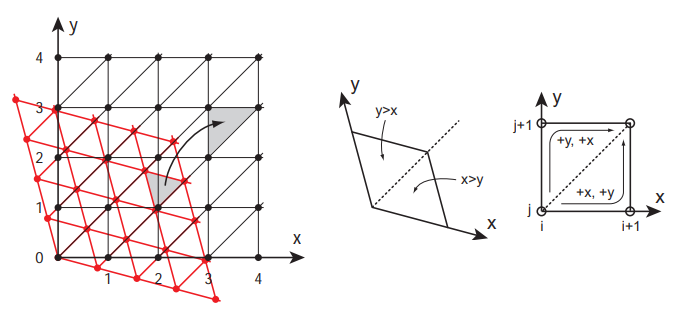
\includegraphics[scale=.5]{skewed grid}
			\captionof{figure}{Skewing in two-dimensional space and determining the cell containing a point. \cite{simplex-demyst}}
			\label{fig:fig9}
		\end{minipage}
		
		The traversal scheme for a two-dimensional simplex is built around this triangular method. If the x and y coordinates are known, then all that is needed is to determine which of the two simplices the point lies in. If x > y, the corners become (0,0), (1,0) and (1,1), else the corners are (0,0), (0,1) and (1,1). To traverse this, only one step in the x and one step in the y is needed, but in a different order for each of the simplices. This technique can then be generalized to any arbitrary amount of N dimensions \cite{simplex-demyst}. While Perlin noise has many advantages over the classical Perlin noise, it has a different visual characteristic, making it difficult to directly replace or compare the two. 
		
		\begin{minipage}{\textwidth}
			\centering
			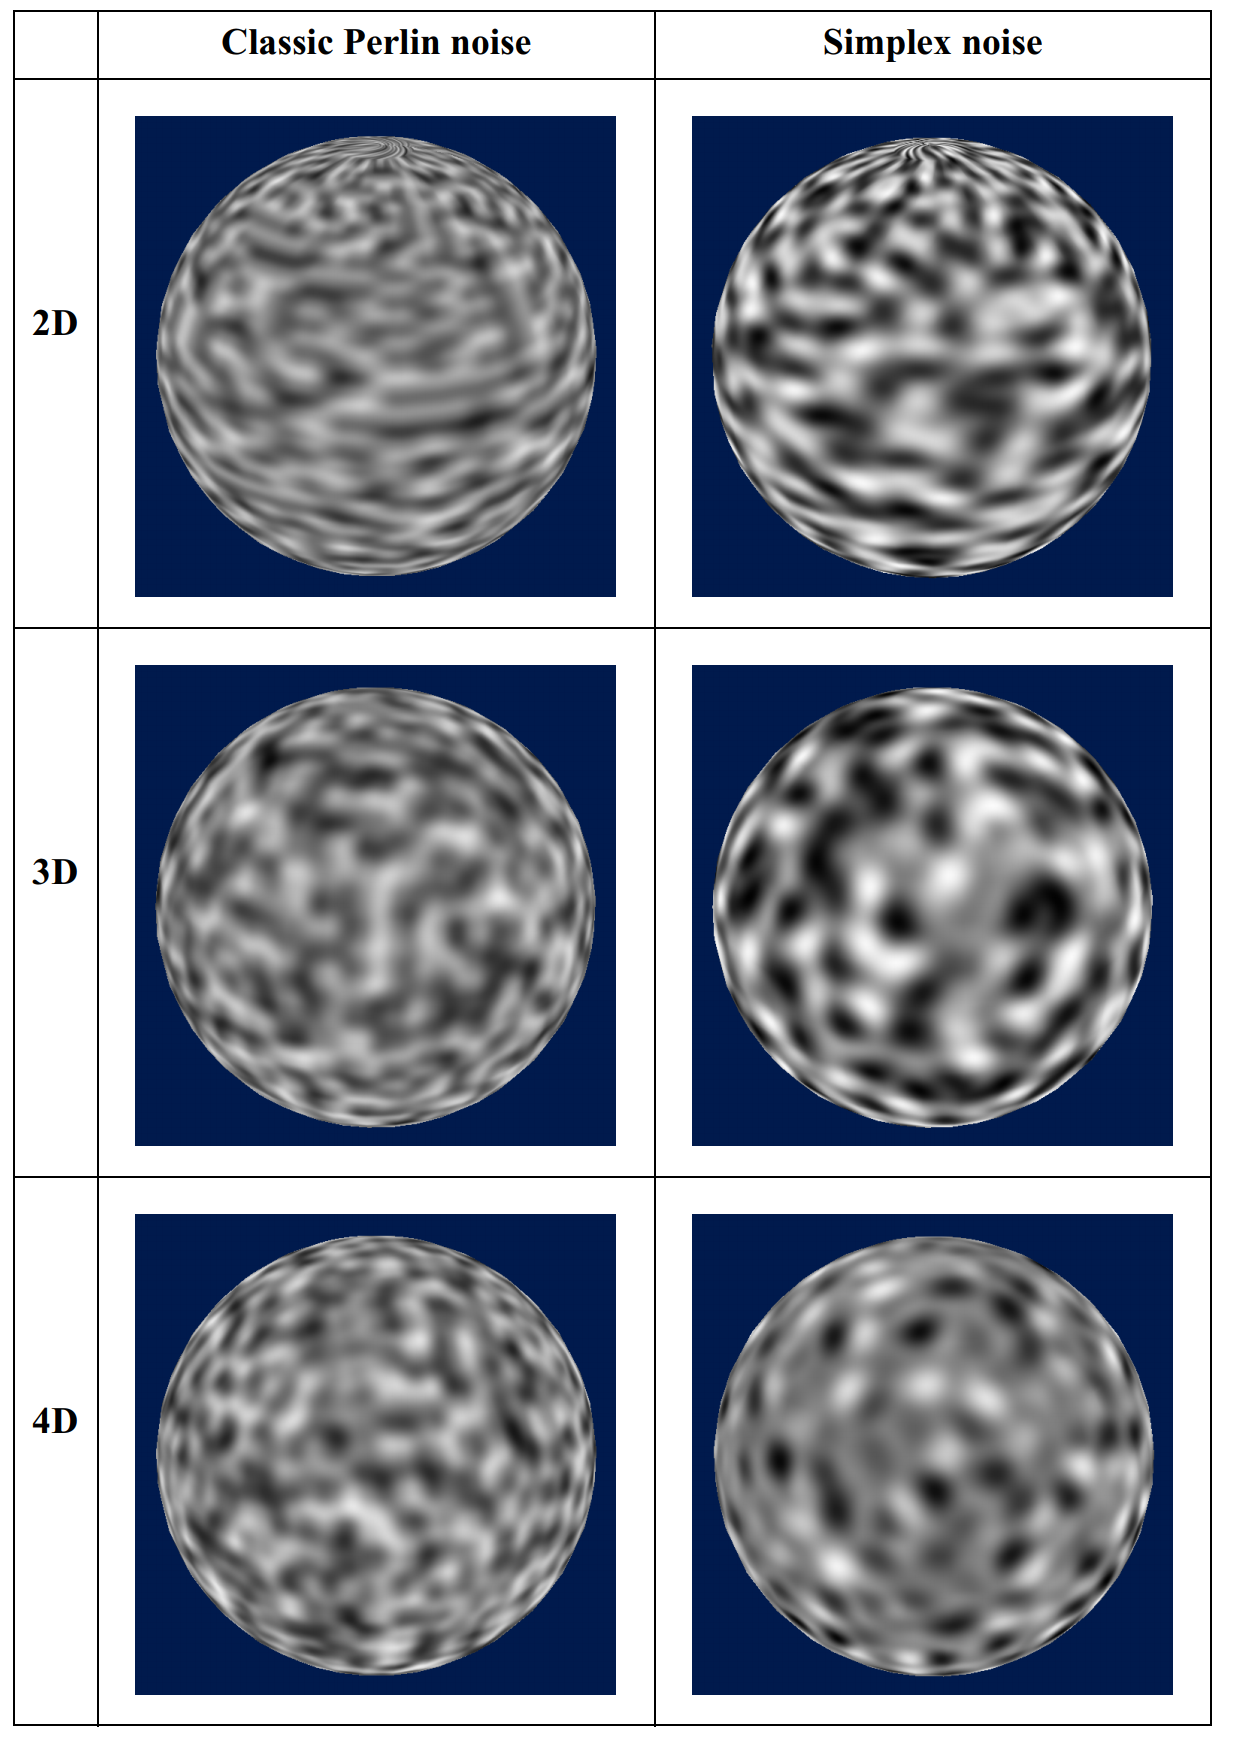
\includegraphics[scale=.25]{perlin vs simplex}
			\captionof{figure}{A comparison of Perlin and Simplex noise \cite{simplex-demyst}}
			\label{fig:fig4}
		\end{minipage}
	
		However, with additional modification using multiple layers or octaves, Simplex noise will run much more computationally efficiently, as well as replicating the visual quirks of Perlin noise. 
		
		In addition to the advancements in noise generation, rendering techniques associated with procedural generation have had advancements as well. For example voxel-based terrain has had advances in both the front and back-end of the algorithms. Voxel-based rendering methods often use a marching cubes algorithm to both smooth voxel surfaces and increase run-times. A modified version of this algorithm was created to facilitate faster implementation and design of a level-of-detail algorithm. Some of the difficulties of this revised implementation of the Marching Cubes algorithm involved finding a suitable compression technique for the voxel map, as for larger terrains, voxel mapping will quickly grow beyond the limits of addressable memory. In addition, limiting the density of vertices, triangles and individual meshes through a level-of-detail system ensures the higher rendering performance of this revised algorithm. 
		
		The modified Marching Cubes combined with a Transition Cubes algorithm provides a method for stitching together voxel-based meshes and eliminating seams. Rendering the areas of a terrain at different detail layers allows for efficient usage of processing power, but introduces the problem of seams between the cells. This problem can be shown in \autoref{fig:voxel-artifact}. 
		
		\begin{minipage}{\textwidth}
			\centering
			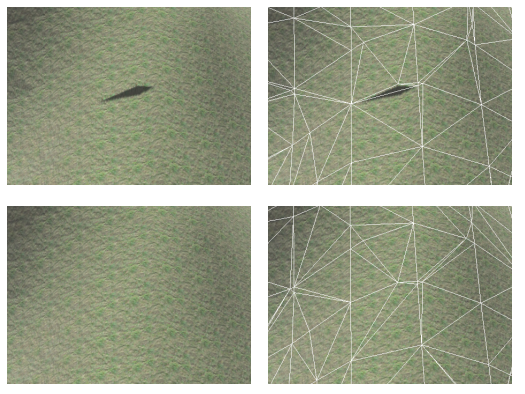
\includegraphics[scale=.75]{voxel-seam}
			\captionof{figure}{A shadow artifact fixed with transition cells \cite{10.5555/1925140}}
			\label{fig:voxel-artifact}
		\end{minipage}
		
		The Transition Cubes method developed in this paper utilizes transition cells inserted in between ordinary cells of a voxel map. This efficiently generates the triangles to connect terrain blocks rendered at different levels of detail, as modifications to one level of detail means that all levels must be adjusted to remain consistent, with the mapping of these different layers shown in \autoref{fig:voxel-layered-mapping}.
		
		\begin{minipage}{\textwidth}
			\centering
			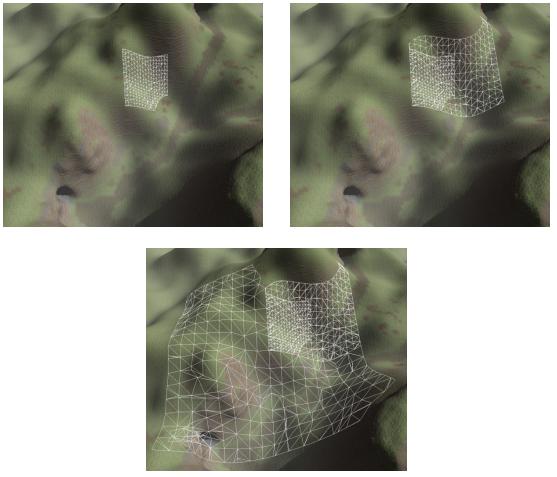
\includegraphics[scale=.75]{voxel-detail}
			\captionof{figure}{Layered resolution details of voxel meshes \cite{10.5555/1925140}}
			\label{fig:voxel-layered-mapping}
		\end{minipage}
		% URL holder http://transvoxel.org/Lengyel-VoxelTerrain.pdf
			
	\vspace{10pt}
	\let\clearpage\relax
	\chapter{Summary}
		
		While procedural generation has a background based in signals processing and mathematics, its usage has extended far beyond these fields in the creation of procedurally generated worlds, stories, characters and more. The procedural generation of geological formations in particular is a difficult problem, as rendering and storing the terrain data in memory proves to be a challenge for any approach of procedural generation. In recent years, the voxel approach has supplanted previous techniques and has become more widespread. However, the fundamental algorithms and processes to create noise have remained largely the same, with improvements. Some of these techniques include Perlin noise, fractal geometry and cellular automata. These techniques have been used to create different sorts of maps in attempts to create two and three-dimensional landscapes. To render the data created from these processes, image-based, polygonal and voxel techniques have been applied, with varying strengths and weaknesses. Image-based techniques have the advantage of low computational requirements and simplicity of implementation, but have the drawbacks of being reliant on either a pre-determined, procedurally generated image, or having an excess of pseudo-random algorithms always running in the background. In contrast, while polygons are a common method for rendering non procedurally generated games, it has several drawbacks with a randomly created space. Interpreting the data from this space becomes a challenge, as well as creating more three-dimensional structures, as polygons have difficulty in creating certain slopes and landscape geometries. Voxels alleviate the problems in geometric representation, but come with the downsides of excessive processing and memory usage, in addition to having issues with tiling. However, for all of these methods, several advancements have been made to mitigate or address these issues. 
	
	\newpage
	\renewcommand{\bibname}{References}
	\bibliographystyle{plain}
	\bibliography{refs} % Entries are in the "refs.bib" file
		
\end{document}